\documentclass[twoside,single]{lion-msc}

\title{Research Proposal \\ \small{\textbf{Finding the Magnetic Field in Cool Core Filaments}}}
\author{B.J. Jung}
\studentid{s1499440}
\supervisor{J.B.R. Oonk; F. Snik}
\corrector{J.M. van Ruitenbeek}
\major{Physics and Astronomy}
\affiliation{Leiden Observatory, Leiden University}
\address{P.O. Box 9513, 2300 RA Leiden, The Netherlands}

\begin{document}

\maketitle



\abstract{
    ABSTRACT
}



\chapter{Introduction}

    \par In recent years a lot of progress has been booked in terms of understanding AGN (active galactic nuclei) feedback into the intracluster medium (ICM) and its effects on galaxy evolution and morphology. Astronomers have not only been able to distinguish different modes of energetic transfer within the feedback, but have also come up with convincing observational evidence for the presence of these modes within various galaxies and galaxy clusters \citep{Fabian2012}. Nevertheless, several problems concerning details of the models persist. \\
    In a paper that was recently published in the Monthly Notices of the Royal Astronomical Society, A.C. Fabian and his team presented an extensive analysis of new HST data of the brightest cluster galaxy (BCG) NGC4696, exhibiting filaments of gas where radiative cooling seems to be suppressed \citep{Fabian2016}. Although optical characterization and velocity measurements suggest that this suppression is caused by interactions with a magnetic field, direct observational evidence supporting the presence of such fields has yet to be presented. This proposal suggests to study the presumed magnetic fields within the gas filaments at the center of the Centaurus galaxy cluster by means of polarimetric analysis of data taken by the VLT's FORS2 instrument during May 2011. For this purpose different techniques can be utilized, which will be explained in the upcoming sections. Before discussing the methods, however, the following section will give a brief overview of the current status of research into cool-core clusters. \\
    
        \begin{figure}[ht]
      \centering
        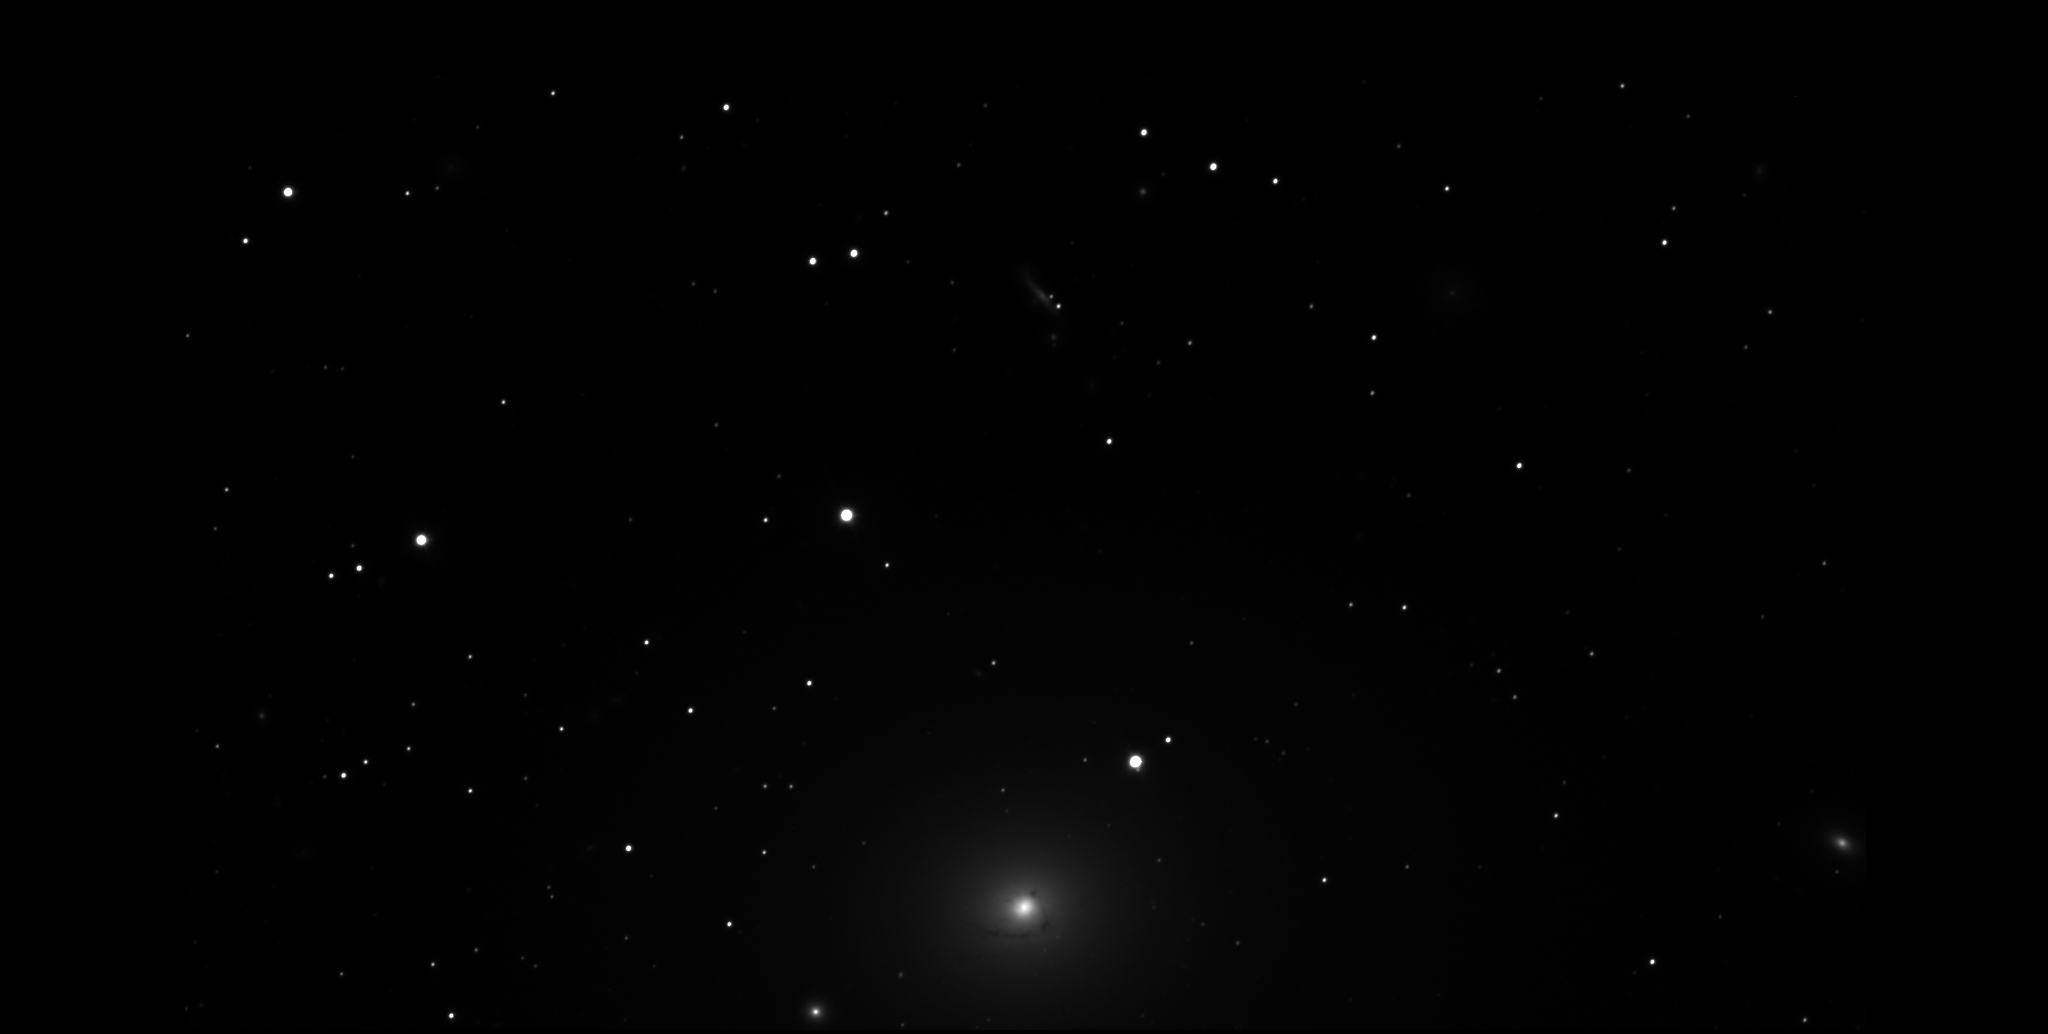
\includegraphics[width=0.9\textwidth]{NGC4696.jpeg}
      \caption{\textit{An image of the Centaurus Cluster taken with the VLT during May 2011. The brightest cluster galaxy NGC4696 is visible in the lower center of the image. Close inspection reveals that the galaxy is surrounded by filaments of gas, suspended around the galaxy center.}}
      \label{fig:NGC4696}
    \end{figure}
    
    
    
\chapter{Theory}    
    
     When astronomers first looked at galaxy clusters in X-ray during the seventies, one curious property immediately caught their eye: although several of these galaxies showcased the existence of central regions with high density and low entropy, the radiative cooling times of the corresponding gas lay well below the Hubble time \citep{Fabian1977, Lea1973, Cowie1977, Mathews1978}. Initially this discrepancy led astronomers to believe that there exists some form of a \textit{cooling flow}, in which gas at the cluster core cools hydrostatically, subsequently compresses under the weight of surrounding hot gas and is then finally replaced by an inflow of such surrounding hot gas (the so-called \textit{cooling flow model}). However, a series of observations conducted in the optical regime eventually lead this model to be discredited. First of all, star formation rates and several molecular abundances associated with cooling flows could not be reproduced \citep{McNamara1989, Edge2001}. Additionally researchers discovered disparities between the mass deposition which could be predicted classically and which could be inferred spectroscopically \citep{Makishima2001}. And lastly, grating spectra acquired by the XMM-Newton telescope revealed that gas in central regions does not cool at the rates predicted by the cooling flow model \citep{Peterson2001, Peterson2003, Tamura2001, Xu2002}. \\
    
    The collective disagreement between theory and observations eventually lead astronomers to conceive of new models which might explain the stable nature of the ICM gas. Most of them looked at ways in which energy might be transferred between AGN's and surrounding gas structures --- something which had not been taken into account within the old cooling-flow model. Among those mechanisms considered were:

    \begin{enumerate}
            \item conduction \citep{Zakamska2002}
            \item central AGN heating due to the combined effect of cosmic ray-ICM interactions and conduction \citep{Guo2007}
            \item Weak shocks induced by buoyant gas bubbles \citep{Mathews2005}
            \item a combination of sound waves and conduction\citep{Ruszkowski2003}
            \item a combination of turbulence and conduction\citep{Dennis2006}
        \end{enumerate}
    
    In the end the search for novel explanations of observed ICM gas features resulted in a change in nomenclature from cooling-flow clusters to \textit{cool-core} clusters. Thus far two different categories of AGN feedback within cool-core clusters have been studied \citep{Fabian2012}. The first one, called the \textit{radiative} or \textit{quasar} mode, deals with feedback mechanisms in which a very luminous central AGN transfers energy directly by means of radiation pressure or by means of interactions via 'winds' of matter surrounding the AGN. The other mode (called the \textit{kinetic} mode) concerns itself with less energetic active galactic nuclei which transfer mechanical energy via processes involving radio-emitting jets. \\ 
    
    \par Acquiring direct observational evidence for the radiative mode has proved to be difficult to obtain due to the problem of concealing gas clouds which typically surround young energetic active galactic nuclei. Nevertheless several efforts to detect ICM winds have come up with promising results by studying X-ray absorption \citep{Tombesi2011, Rupke2011}. Evidence for the kinetic mode seems much more abundant and has been frequently observed in the form of gaseous bubbles arising buoyantly from the active galactic nuclei as a byproduct of jet activity \citep{Churazov2000, Churazov2000a, McNamara2000}. One remarkable feature about this 'bubbling action' of active galactic nuclei is that it can give rise to large-scale nebulosities of emission-line filaments. In a Nature paper published in August 2008, A.C. Fabian and his team further investigated several of such filaments in the neighborhood of NGC1275 and came to the surprising conclusion that they are somehow stabilized against gravitational collapse \citep{Fabian2008}. By considering the radial length and mass of the filamentary structures, as well as their experienced gravitational acceleration, they inferred that the stabilization would most likely be caused by the influence of a tangential magnetic field component of strength $24 \mu G$. More recent observations of filaments surrounding the Centaurus cluster BCG NGC4696 reveal a similar scenario for tangential magnetic field strengths of $75 \mu G$. \\
    In order to establish the validity of claims about magnetic fields within ICM filaments, it is pivotal that we acquire direct observational evidence of these presumed magnetic fields. Polarimetry might provide the means to do so by allowing for measurements of the degree of polarization in received radiation as an effect of dust particle alignment with the fields.
    
    
    
    
\chapter{Methodology}    

    In order to observe the magnetic fields present within the gas filaments surrounding NGC4696, we will analyze polarimetric data acquired by the FORS2 instrument at the VLT. This instrument consists of a retarder waveplate followed by a Wollaston beam splitter, allowing for polarimetric demodulation schemes as described by S. Bagnulo and his team in his 2009 paper on stellar spectropolarimetry techniques \citep{Bagnulo2009}. We first define the following quantity:
    
    \begin{equation}
        G(\alpha, \gamma) = \frac{S(\alpha, 0^{\circ}, \gamma) - S(\alpha, 90^{\circ}, \gamma)}{S(\alpha, 0^{\circ}, \gamma) + S(\alpha, 90^{\circ}, \gamma)}
    \end{equation}

    where $S(\alpha, \beta, \gamma)$ stands for the signal received after rotating the retarder waveplate over an angle $\alpha$, after rotating the Wollaston prism (or more generally, the polarizer) over an angle $\beta$ and where the phase shift introduced by the retarder waveplate is given by $\gamma$. Then it holds true that for the three different Stokes parameters Q, U and V:
    
    \begin{align*}
        \mathcal{G}^{[j]}_{Q} &= G(\alpha = (j-1) \times 45^{\circ}, \gamma = \pi) \\
        \mathcal{G}^{[j]}_{U} &= G(\alpha = 22.5^{\circ} + (j-1) \times 45^{\circ}, \gamma = \pi) \\
        \mathcal{G}^{[j]}_{V} &= G(\alpha = -45^{\circ} + (j-1) \times 90^{\circ}, \gamma = \pi) \\
    \end{align*}

    Furthermore, the redundancy in the measurements of the different parameters enables one to make partial corrections for instrumental effects by means of the \textit{difference method} or the \textit{ratio method}, both of which additionally allow for quality checks by means of null parameters. \\
    Our research sets out to apply these various methods and checks in order to establish the polarization degrees of the gas filaments around NGC4696 as accurately as possible.
    
    
   
\chapter{Expected Achievements}

    The goal of our research is to create a map of the polarization degrees of gas filaments within the Centaurus galaxy cluster and to analyze the influence of magnetic fields on the stability of these filaments. In doing so, we hope to shed new light on the processes involved in AGN feedback as well as provide additional information about the gas dynamics in cool-core galaxies. Since studies have shown that a significant amount of galaxies fall into the cool-core regime (ranging from 40\% to 70\% depending upon the chosen samples of observations) \citep{Hudson2010, Chen2007, Sanderson2008}, this might prove relevant for future research within the field.
    
    
 
\chapter{Data management}

    For the purpose of this research we'll use polarimetric data taken using the FORS2 instrument of the VLT during May 2011. This data is freely available and can be donwloaded from the ESO science website. Graphs and images which are created as a result of the research are stored locally, but will be regularly uploaded to an external hard drive (i.e. minimally once per week). At the end of the project, data can be uploaded to one of the Observatory's data repositories if necessary.
    
    
    
\chapter{Skills and Planning}
    
    This section contains a non-exhaustive list of my current abilities pertaining to the project, as well as strategies for their development. At present my skills and knowledge consist of the following:
    
    \begin{enumerate}
        \item Galactic dynamics - basic
        \item Imaging polarimetry - elementary
        \item Astronomical data analysis - basic
        \item Writing - intermediate
        \item Programming - basic
    \end{enumerate}
    
    I expect to be able to improve upon my knowledge with respect to all of the above facets during my work on this project. 
    
    
    
\chapter{Planning}

    \begin{figure}[h]
      \centering
        \includegraphics[width=0.9\textwidth]{gantt3.pdf}
      \caption{\textit{A gantt chart showing the outline of the project's time schedule. During March and the beginning of April, data will be polarimetrically demodulated, after which most time will be spent on the astrophysical interpretation of the derived results. The project report will be written down during May, which leaves one month of latency time if proven necessary.}}
      \label{fig:gantt}
    \end{figure}

    For a global overview of the planning surrounding this project, I refer to the gantt shown in figure \ref{fig:gantt}.









%----------------------------------------------------------------------------------------
%	BIBLIOGRAPHY
%----------------------------------------------------------------------------------------
%to compile succesfully use:
%    pdflatex filename (with or without extensions)
%    bibtex filename (without extensions)               %compile library file
%    pdflatex filename (with or without extensions)
%    pdflatex filename (with or without extensions)
%

\renewcommand\refname{}
\bibliographystyle{plainnat}
\bibliography{brpref3.bib}





\end{document}
